%********** Chapter 1b, the new chapter 2 **********

\chapter{Fortune Teller}\label{ch:fortune}\index{Fortune Teller}\index{projects!Fortune Teller}

%\section{Introduction}

This chapter dives into programming with the first project, a program that generates a user's lucky number and uses it to predict the user's fortune\index{Fortune Teller}.  The program works by asking the user for a favorite and a disliked number and then combines them to create a lucky number and a fortune based on the lucky number.  As we'll see the program is fairly simple, but also very flexible. It's possible to include all sorts of user input and fortunes.

The Fortune Teller program introduces the following elements of programming:
\begin{tight_itemize}
   \item Comments\index{comments}
   \item Variables\index{variables}
   \item Input/output (I/O)\index{I/O}
   \item Mathematical Expressions\index{Expressions}
   \item Conditionals:\index{conditionals} \cf{if}
   \item Libraries\index{libraries}
\end{tight_itemize}

Comments are sections of code used by the programmer to make the program more readable, but that are ignored by the computer, that is they are comments about the code from one programmer to another.   Variables are used to store the data used by a program.  Input is data that comes into a program from another source -- typically the keyboard or a file.  Output is data that is sent from a program -- typically to the screen or to a file.  Mathematical expressions let the program perform mathematical operations.
Conditionals are specialized commands that allow a program to make a ``decision'' -- doing one thing under some conditions and doing something else under other conditions.  Without conditionals programs would always do exactly the same thing.   
Libraries are sets of prewritten code that are included in a program.  As the Fortune Teller project demonstrates, a basic understanding of these elements is sufficient for writing  fairly sophisticated and interesting programs.

\section{The Program}

Listing~\ref{listing:FortuneTeller} presents the code for the Fortune Teller.  Notice that the program is actually fairly short -- only 38 lines long -- and many of the lines are comments.  When entering the code do \emph{not} enter the line numbers along the left side of the program.  Those are just for reference.  As the program is entered, try to figure out what the commands do.  Most will be difficult to understand at this point, but some of them may make sense.

%\begin{figure}
\begin{minipage}{\textwidth}
\begin{lstlisting}[language=C++,numbers = left, xleftmargin=4.0ex, basicstyle=\small,emph={num_objects,move,current_player},emphstyle = \color{\mycolor},
showstringspaces=false,
caption = {The code for the Fortune Teller.  When entering this program, do not enter the line numbers.  Keywords (also known as reserved words) are in bold, comments are in italics, and variables are colored maroon.}]
      /* The Fortune Teller -
       * a simple program introducing some
       * fundamental programming concepts.
       */
#include <iostream>  // include a library
using namespace std;
int main()  // main() starts the program
{
	// ----------------- Variable declarations ------------------------
	int favorite;  // create a variable to store the favorite number
	int disliked;  // create a variable to store the disliked number
	int lucky;  // create a variable to store the lucky number
	// ----------------- Get user input -----------------------------
	cout << "Enter your favorite number (no decimals): ";  // output
	cin >> favorite;                         // user input
	cout << "Enter a number you don't like (no decimals): ";
	cin >> disliked;
	// Next calculate the user's lucky number
	lucky = (favorite * disliked) % 10;
	cout << endl << "Your secret, lucky number is: " << lucky << endl;
	if(lucky < 0){  // conditional, values less than 0
		cout << "Try to be less negative." << endl;
	}
	if(lucky >= 0 && lucky < 5){ // 0 to 4 inclusive
		cout << "Think bigger!" << endl;
	}
	if(lucky >= 5 && lucky < 9){  // 5 to 8 inclusive
		cout << "Today you should embrace technology." << endl;
	}
	if(lucky == 9){     // exactly 9
		cout << "Today is your lucky day!" << endl;
	}
	// ------- Code to help the program exit "gracefully" --------
	cin.ignore();
	cout << "Press enter to quit." << endl;
	cin.ignore();
	return 0;
}
\end{lstlisting}\label{listing:FortuneTeller}
\end{minipage}
%\caption{The code for NIM.  When entering this program, do not enter the line numbers.}
%\end{figure}\label{fig:NIM1}



\begin{wrapfigure}{R}{0.5\textwidth} \vspace{-0.5cm}\framebox[\linewidth][l]
{\parbox{0.96\linewidth}
{\textbf{Using Comments} \\
Good code contains many comments.  Comments make code much more readable, which makes it easier to understand, modify, and expand a program.  Most of the programs presented in this text are seriously \emph{under}-commented so that the reader can add their own comments as the meaning of the code becomes clearer.  This is done to encourage the reader to add comments to the code.  It also saves space and reduces the amount of text to copy (although the comments can be skipped when the program is entered).  Software companies often have rules that specify how code must be commented (for example, requiring a comment before every function).  If you are using this text as part of a course, there are likely requirements that each program start with a block comment containing information like your name, the assignment number, and your section.
}}
\vspace{-1.5cm}
\end{wrapfigure}

Once the entire program has been entered, compile it.  Depending on how carefully the program was entered, the compiler may generate some error messages.  Try to fix them and compile the program again.  Read the compiler error messages carefully; at the very least, they report the line that the error occurred on.  Because one error may hide another error, it may take several iterations of compiling and fixing errors before the program compiles successfully.  More detailed suggestions on how to fix a program that's not compiling or running properly are presented in the interlude following this chapter.

Once the program compiles, run it a few times to generate different fortunes.  While running the program compare the program's output to the program's code.  It should be possible to recognize what many of the program statements do by seeing how the program runs.  

Running the program will also reveal that it has some shortcomings.  It doesn't tell the user what the program does.  The output messages are not always clear.  There's a fairly limited number of fortunes.   These are shortcomings that we will eventually want to fix.  But before modifying the program it is necessary to discuss its important elements and to analyze how it works.

\subsection{Comments}\index{comments}

 A \emph{comment} is part of a program that has no effect on how a program runs, but that makes a program more readable for humans, either by explaining what a section of code does or by structuring the program so that it is easier to read.  For example, the comments on lines 5 and 7 explain those lines of code and the comments on lines 9, 13, and 33 serve to break the program into three easy-to-identify blocks.  

Comments are defined in C++ in two ways, either using two slashes // (e.g., lines 9, 10, and 11) or with a /* ... */ pair (lines 1-4).  When two slashes are used, everything from the slashes to the end of the line is a comment.  For example, the first part of line 10, up to the slashes, is regular code and the rest, after the slashes, is a comment.
When a /* ... */ pair is used, everything from the starting /* to the ending */ is part of the comment.  For example, the block of text on lines 1-4 is one large comment.

\subsection{Variables}\index{variables}

Programs often need to keep track of information -- the program's \emph{data}.  For example, the Fortune Teller needs to know the user's favorite, disliked, and lucky numbers.  Programs use \emph{variables} to keep track of this information.  A variable can be thought of as a named box that stores a piece of data.  Figure~\ref{fig:variables1} illustrates this idea.

\begin{wrapfigure}{R}{0.5\textwidth}\vspace{-0.5cm} \framebox[\linewidth][l]{\parbox{0.96\linewidth}
{
\codefont{Naming Variables} \\
The rules for valid variable names are fairly simple.  Variable names can use letters, underscores (\_), and digits, but cannot start with a digit and must contain at least one letter.   They may not be a reserved word, such as \codefont{if}, \codefont{int}, or \codefont{main}.  In the code listings reserved words are shown in bold.  Case matters: \codefont{X} is not the same variable as \codefont{x}.  Thus, legal variable names include: \codefont{X}, \codefont{a\_variable}, and \codefont{variable7}, but \emph{not} \codefont{7variable} (starts with a digit),
% \codefont{\_123} (doesn't contain a letter),
or \codefont{do} (a reserved keyword).  There are a number of conventions for choosing variable names and software companies often enforce the use of a particular convention.  Several  conventions are used in this text to demonstrate the range of variable naming styles.
}   }
\vspace{-0.4cm}
\end{wrapfigure}

In addition to its name, each variable must have a \emph{type}\index{type}.   The type defines what kind of data can be stored within a variable.  The Fortune Teller program has three variables: \cf{favorite}, \cf{disliked}, and \cf{lucky}, all of which have the same type: integer or \cf{int}.  There are three main reasons why a program  must know the type of a variable.  First, the type determines how ``big'' a variable's box is -- literally, how much of the computer's memory it takes up.  

\begin{figure}
%\centerline{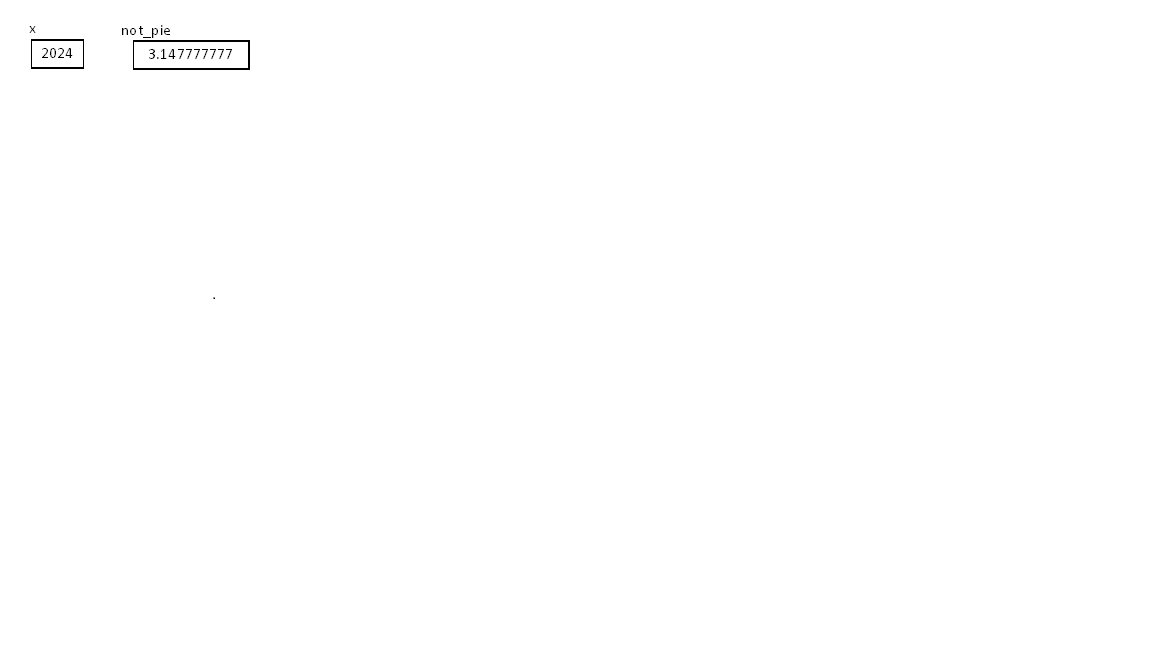
\includegraphics[width=9cm,height=3cm]{images/variables.bmp}}
\setlength{\unitlength}{1cm}
\begin{picture}(10,2)

\linethickness{0.3mm}

\put(4.2,1.1){376}
\put(4,1.7){\codefont{X}}
\put(7.2,0.9){4.17222}
\put(7,1.5){\codefont{not\_pi}}

\put(10.2,0.7){f}
\put(10,1.3){\codefont{character\_variable}}

\color{\mycolor}{
\put(4,1){\line(1,0){1}}  % bottom
\put(4,1.5){\line(1,0){1}} % top
\put(4,1){\line(0,1){0.5}} % left
\put(5,1){\line(0,1){0.5}} % right

\put(7,0.8){\line(1,0){2}}  % bottom
\put(7,1.3){\line(1,0){2}} % top
\put(7,0.8){\line(0,1){0.5}} % left
\put(9,0.8){\line(0,1){0.5}} % right

\put(10,0.6){\line(1,0){0.5}}  % bottom
\put(10,1.1){\line(1,0){0.5}} % top
\put(10,0.6){\line(0,1){0.5}} % left
\put(10.5,0.6){\line(0,1){0.5}} % right
}

\end{picture}
\caption{Variables can be thought of as boxes with a name that hold a value.  Different types of variables correspond to different-sized boxes. }
\label{fig:variables1}
\end{figure}

Second, the type determines how to interpret the data stored in the variable.  At the lowest level, data is stored in a computer as a binary\index{binary} number.  \emph{Binary numbers} are numbers that are written using only the digits 0 and 1, instead of the digits 0 to 9 we are used to (see Appendix~\ref{appendix:binary}).  
Computers use binary numbers because they can use \codefont{off} and \codefont{on} to represent 0 and 1.  However, different data types use the 0's and 1's in different ways.  The computer needs to know the type of the variable to know how to interpret the 0's and 1's stored in the variable.

Third, the type tells the program how operations should be applied to the data stored in the ``box.''  For example, when division is applied to two integers, the answer is an integer and the remainder is ignored, but when division is applied to two real numbers the answer is also a real number.

Variables are declared using statements like:\\
\codefont{
\emph{type} name;\\
\emph{type} name1, name2, name3;\\
\emph{type} name4 = \emph{value};\\}
where the \codefont{\emph{type}} is the type of the variable to be created, \codefont{name} is the name of the ``box,'' and \codefont{\emph{value}} is the value the variable initially stores.  
The second of these statements demonstrates that multiple variables can be declared in one statement, as long as all of the variables have the same type.  The third statement shows that variables can be assigned a value as soon as they are created.
For the Fortune Teller, only variables of type \emph{integer}\index{integer}\index{type!int@{\cf{int}}} (abbreviated as \codefont{int} in C++\footnote{Computer languages and computer programmers often rely on abbreviations.}) are used.  Other types are introduced in later chapters, and Section~\ref{appendix:types} in Appendix A has a list of the most commonly used types in C++.  In the Fortune Teller variables are declared (i.e., created) on lines 10-12.

Variable names are selected by the programmer, subject to C++'s naming rules (see the text box Naming Variables).   Giving variables meaningful names makes code easier to read and understand. For example, the variable holding the user's favorite number is named \cf{favorite}. 

\subsection{Input and Output}\index{I/O}

In C++, input and output to a program goes through objects known as  \emph{streams}\index{streams}.  A stream object represents a device that can send or receive data using input and output operations.  For example, \codefont{cout} is a stream object representing the computer terminal, so sending data to \codefont{cout} results in the data being displayed on the screen.  

Data is sent to or received from streams using stream \emph{operations}.  Most stream operations have a similar structure: they define the stream to be used and the type and/or amount of data to be sent or received.  In C++ the most common stream operators are $<<$ and $>>$, which represent sending data to or receiving data from a stream.  For example, the statement:\\
\codefont{cout $<<$ "Hello, world!";}\\
sends the data in the string ``Hello, world!'' to the stream \codefont{cout}. Thus, this command prints the words ``Hello, world!'' on the screen.  Many other streams and stream operations exist and will be introduced throughout the text.  A list of the most common stream operations is included in Section~\ref{appendix:iostream} of Appendix A. 

\subsection{Expressions}\index{expressions}

Mathematical expressions are simply used to perform calculations within a program.  Their general format is:\\
\cf{x = \emph{mathematical expression}}\\
where \cf{x} is a variable and the \emph{mathematical expression} is build from variables, numbers, and mathematical operators (+, -, etc.).  The variable \cf{x} is assigned the value that is calculated on the right hand side of the expression.  

There are a two things to be careful of when creating mathematical expressions in C++: \emph{order of operations} and \emph{types}.  Order of operation is the order that mathematical operations are applied in a compound mathematical expression like:\\
\cf{x = y + 7 * 8 - z}\\
C++ uses the standard rules for order of operation (multiplication and division before addition and subtraction; addition and subtraction are performed left to right; etc.).  So, in the previous expression \cf{7 * 8} would be performed first.  %However, C++ includes a number of useful, but possibly unfamiliar, mathematical operations (See Section~\ref{appendix:operators} of Appendix A) whose

C++ has many mathematical operators, including basic operators like addition (+), subtraction (-), and division ($\backslash$), and more unusual, but useful, mathematical operations like increment (++) and decrement (- -).  More operators will be introduced as they are needed in later chapters.  Section~\ref{appendix:operators} of Appendix A has a list of the commonly used C++ operators.  Because the order of operations of these operators may not be familiar it is a good idea to use parentheses to force operations to take place in the desired order.  Including parentheses also makes expressions easier to read.

Depending on the types involved mathematical expressions can sometimes give unexpected results.  For example, the code:\\
\cf{
int x = 8;\\
cout << x / 10;\\
}
prints the number \emph{0}.  The variable \cf{x} and number 10 are both integers, so C++ treats the answer as an integer and the value 0.8 (possibly the expected answer) is \emph{truncated}\index{truncation} to zero.  There are a number of ways to avoid this problem.  For example, if the code were rewritten as:\\
\cf{
int x = 8;\\
cout << x / 10.0;\\
}
including the decimal on 10.0 tells C++ to treat the answer as a decimal and the code will print 0.8.  The issue of types in mathematical operations is examined in more detail in later chapters when more types (besides \cf{int}) have been introduced.

\subsection{Conditionals: \cf{if}}\index{conditionals}

Conditionals allow a program to choose between two (or more) options.  The options are often referred to as \emph{branches}.  One of the most common conditionals is the \emph{if}\index{if@{\cf{if}}} statement.  All conditionals have a \emph{condition}\index{condition}: if the condition is true the computer executes (i.e., runs) one block of code, if the condition is false the program skips that block of code, and may run a different block of code instead.  The format of an if statement is:\\
\codefont{
if(\emph{condition}) \{\\
\hspace*{0.5cm}Execute this block of code\\ 
\hspace*{0.5cm}if the condition is true\\
\}\\
Always executed\\
}
Notice that the condition is inside the parentheses after the \codefont{if}.  The blocks of code within the if statement is denoted in two ways: it is surrounded by curly braces, \{ and \}, and the code is indented.  The curly braces define the block of code within the if statement for the computer.  Whereas the indenting makes it easier for programmers to quickly identify the code that is part of the if statement.  Indenting is not required, but blocks of code within curly braces should \emph{always} be indented because it makes the code much easier to read.  


C++ also has an if-else statement and a switch statement both of which are slightly more complex conditionals, covered in later chapters.  These conditional statements are also summarized in Section~\ref{appendix:conditionals} of Appendix A.  

Conditions used in conditional statements are typically written as \emph{Boolean} expressions.  Boolean expressions are logical expressions whose value is either \emph{true} or \emph{false}.  Boolean expressions are constructed by using comparison operators like less than ($<$), greater than ($>$), equal to ($==$), and not equal to ($!=$).  Boolean expressions also use the logical operators AND (which is written as $\&\&$ in C++), OR (written as $||$), and NOT (written $!$).  For example, the 
statement:\\
\cf{
x < y || y > z \\
}
is a condition that is true \emph{if x is less than y OR if y is greater than z}. 
Commonly used comparison and logical operators are introduced in later chapters and summarized in Section~\ref{appendix:Boolean} of Appendix A.  

Although Boolean expressions evaluate to true or false, C++ takes a shortcut and uses a \cf{0} for false and a \cf{1} for true.  For example, a command like:\\
\codefont{cout << (6 < 8) << endl;}\\
will print a 1 because 6 is less than 8 and C++ uses a 1 for true and 0 for false.  Similarly, the expression \codefont{6 > 8} would produce a 0.  

More generally, in C++ any nonzero value is treated as true.  This means that non-Boolean expressions can be used in conditions.  For example, the condition in an if-else statement could be \codefont{x - 7}.  This would be interpreted as ``false'' for \codefont{x = 7} because \codefont{x - 7} would be 0.  It would be interpreted as ``true''; for any other value of \codefont{x}.  However, using mathematical operations in the place of comparisons is generally a poor idea because it makes the code less readable.  For example, understanding the condition \codefont{x - 7} is harder than understanding \codefont{x != 7} even though both test the same condition.  


\section{Analysis of the Code}

This section analyzes the code in Listing~\ref{listing:FortuneTeller} line by line.  It explains how the program works and how the statements in the program can be modified or used in other programs.  The goal in analyzing the code is to understand the Fortune Teller program and to understand how the statements used in Fortune Teller can be adapted for writing other programs.

\mysubsubsection{Lines 1-5, 7, and More: Comments}
Because computer programs are generally difficult for humans to read, comments are included to make programs more readable to humans.  In C++ there are three general forms of comments: block comments, full line comments, and end of line comments. 
Lines 1-4 are a single block comment describing the program.  Block comments begin with a /* and end with a */, anything between those two symbols are ignored by the complier.  Note that the extra *'s on lines 2 and 3 are not required, they are there just to make the comment easier to identify.  Programmers often include contextual cues to make different parts of a program easier to see.

\begin{wrapfigure}{R}{0.5\textwidth} \vspace{-0.3cm} \framebox[\linewidth][l]{\parbox{0.96\linewidth}{\codefont{Formatting Programs} \\
For the most part, C++ compilers don't care about formatting: indenting, extra spaces, tabs, and newlines are mostly ignored by the compiler.  However, proper formatting is very important to making programs human-readable.  Proper indenting acts as a visual cue  in much the same way that line breaks, periods, and indenting helps the reader know where sentences, paragraphs, and chapters begin and end in a document.  Reading large blocks of unformatted text is difficult, and reading large blocks of unformatted or badly formatted code is even harder.  The basic rules of good program formatting will be introduced throughout the text.  The first rule is to indent any block of code between curly braces: \{and \}. }   }
\vspace{-0.5cm}
\end{wrapfigure}

Lines 9, 13, and 33 are full line comments.  They break the program into identifiable sections, another form of contextual cue to help programmers understand how the program works.  Because these comments are only one line they can begin with // and automatically end at the end of the line.

Finally, there are lots of short comments throughout the program (e.g., lines 5, 7, 10, and so forth).  Each of these short comments also starts with // and extends to the end of the line.  If you try to add code on the same line after a // the compiler treats it as part of the comment.  These short comments are there to explain what the lines of code do.  Adding comments is a very good programming habit and is strongly encouraged.  

\mysubsubsection{Lines 5-6: \#includes}\index{include}\index{libraries}

Commands starting with a \# sign are \emph{preprocessor directives}\index{preprocessor}.  They are read by the preprocessor, which is one step in the process of compiling the program.  Although there are many different preprocessor directives, this text only covers \codefont{\#include}, which allows the program to access a library.  A \emph{library}\index{library} is a separate file that contains additional code that the program uses.  In this case, the program needs the \codefont{iostream} library\index{iostream@{\cf{iostream}}}, which contains code that defines the \emph{input} and \emph{output} \emph{streams} (hence the name \codefont{iostream}) used to send data to and from the program.  Thus, if a program is going to send text to the screen or to get data from the keyboard (as all of the programs in this text do), it needs  to ``include'' the iostream library.

%The second library this program uses is the \codefont{cstdlib} library\index{cstdlib@{\cf{cstdlib}}}.  The name \codefont{cstdlib} is short for \codefont{C} \codefont{STanDard} \codefont{LIBrary}.  This library contains code that helps with a number of programming tasks.  In particular, the \codefont{cstdlib} includes code for generating random numbers, which the NIM program uses  for generating the computer's move. 

As the number of available libraries grows, it becomes harder and harder to keep track of their names.  Thus, line 6 is used to let the compiler know that we are using the \emph{standard} \emph{namespace}\index{namespace} (``std'' is an abbreviation for \emph{standard}).  Other namespaces exist, but won't be used in this text.   Other libraries will be introduced later in the text.  Section~\ref{appendix:libraries} of Appendix A lists some of the commonly used libraries.

\mysubsubsection{Lines 7-8 and 38: Main}\index{main()@{\cf{main()}}}

The line \codefont{int main()} marks the beginning of the program.  Technically, it defines the beginning of the ``main function.''  Functions will be discussed in later chapters.  For now, it is only important to know that all complete C++ programs start running at main and that C++ programs must have a main function.  

The next line, line 8, is just a \{.   There is a matching \} on line 38, which marks the end of \codefont{main()}, which is also the end of the program.  As noted earlier, C++ uses curly braces \{ and \} to denote blocks of code.  In this case, these braces denote all of the code that is within \codefont{main()}, which is also all of the code in this program.  The code in Listing~\ref{listing:FortuneTeller}  has numerous other pairs of braces that are used to define other, nested blocks of code. Note that each block of code is indented so that it is easier to identify.   

The initial \{ of a block of code can be placed on it's own line, for example, line 8.  Or it can be placed on the proceeding line, for example, line 21 and line 27.  Either of these styles is fine, as long as it's easy to tell where the block of code begins.  The final \} of a block of code should go on it's own line (although technically it doesn't have to) to make it easy to identify the end of a block of code.

\mysubsubsection{Lines 10-12: Variables}\index{variables}

Lines 10-12 \emph{declare} three variables that are used in the Fortune Teller program.  Line 10 declares a variable whose name is \codefont{favorite} and whose type is \codefont{int}. In this case \codefont{int} is short for \emph{integer}, meaning that the variable \codefont{favorite} will store only integer numbers and will never store a decimal value.  
The variable \codefont{favorite} is used to store the user's favorite number. 

Similarly, line 11 declares a variable named \codefont{disliked} of type \codefont{int} and line 12 declares a variable named \codefont{lucky}  of type \codefont{int}.  Initially the code doesn't put any value in these variables, which means that the values are \emph{undefined} -- they could have an integer value.

The final thing to notice about lines 10-12 is that all three of them end with a semicolon.  The semicolon marks the end of a command.  It serves roughly the same purpose as a period in English and ends most commands in C++.  

\mysubsubsection{Lines 14-17, 20, 22, 25, 28, 31, and 34-36: Input and Output (I/O)}\index{I/O}

Lines 14, 16, 20, 22, 25, 28, 31, and 35 are all output commands.  They send data from the program to somewhere else, in this case to the screen.  The first part of an output command (\codefont{cout})\index{cout@{\cf{cout}}} determines where the data will be sent.  The keyword \codefont{cout} represents the \emph{output stream} that corresponds to the computer's screen.  So, using \codefont{cout} will send data to the screen.  Later chapters describe how similar commands are used to send and receive data from files.  Next in the command are the symbols \cf{$<<$} (two less than symbols typed in a row, with no space between them).  The symbols \cf{$<<$} are a pipe operator, they ``pipe'' data to the output.  They are placed between every piece of data that gets sent to the output.

Next comes the data itself.  Typically, output data comes in two forms: \emph{literal strings}\index{literal strings} and data stored in variables.   Literal strings are a string of characters.  They are denoted by double quotes.  Everything within the double quotes is sent directly to the output, not including the quotes themselves.

To print the data stored in a variable, the variable's name is used without any quotes.  The computer automatically prints the data, not the variable's name.  The program uses the variable's type to determine how to display the variable's value.  

In addition to literal strings and data, there are also special signals that can be sent to a stream.  One of these is represented by the word \codefont{endl} (short for ``\emph{end} of \emph{l}ine,'' note that the last character is a lower case L, not a one).  Sending \codefont{endl} to an output stream causes the output to skip to the next line.  

Putting this all together, line 20 will print\\
\codefont{Your secret, lucky number is: \emph{lucky}}\\
where \cf{\emph{lucky}} will be replaced by the value of the variable \codefont{lucky}, and 
the output will be on a new line and followed by a new line.  

%Instead of using \codefont{endl} to create a newline, lines 20, 34, and 36 use the character sequence `\textbackslash n'\index{new line}.  This also inserts a new line into the output, which helps make the output easier to read.  Sequences consisting of a \textbackslash~followed by another character are known as \emph{escape} sequences\index{escape character}\index{escape sequence}.  A few others are \textbackslash t for tab, \textbackslash ' for a single quote,  \textbackslash\textbackslash~for a backslash, and \textbackslash '' for a double quote. 
% To send double quotes to the output  In that case, you use an escape sequence\index{escape sequence}, a pair of characters where the first character is a \textbackslash.  So, to print a literal string containing double quotes you would use a string like \codefont{``\textbackslash``Here's a quote\textbackslash''''}, which would print \codefont{"Here's a quote"} with one set of double quotes.}  

Line 15 is an input command.  It is similar to the output command, but with two changes: the keyword \codefont{cin}\index{cin@{\cf{cin}}} is used instead of \codefont{cout}, and the pipe operator points the other way: \cf{$>>$}.  Input commands take data from a source, such as a keyboard, file, or other device, and store it in a variable.   \codefont{cin} is a stream object representing the keyboard.  So, when the computer reaches a \codefont{cin} command, it pauses and waits for the user to input data at the keyboard followed by the Enter key; nothing happens until Enter is pressed.  The data is then stored in the variable listed in the command.  Thus, when the command: \\
\codefont{cin >> lucky;}\\
is reached (line 15), the computer pauses and waits for the user to type an integer followed by the Enter key.  After the user presses enter, the value they entered is stored in the variable called \codefont{favorite}, making it available to the program.  

\begin{wrapfigure}{R}{0.5\textwidth} \vspace{-0.3cm} \framebox[\linewidth][l]{\parbox{0.96\linewidth}{\codefont{Input Validation}\index{input validation} \\
An important part of programming is recognizing that the user often supplies unexpected input; for example, entering the word \emph{two} instead of the digit 2.  Complete, robust input validation is an important, but difficult topic.  It requires accepting every input in the most general way possible and trying to figure out what the user \emph{really} meant.  To keep the issue simple, the programs in this text assume that the user enters the correct type of value, but not always a valid value.  For example, if the program expects an integer in the range 0-10, we'll assume that the user enters an integer, but not necessarily in that range.}   }
\vspace{-0.5cm} 
\end{wrapfigure}

There are a couple of tricky issues with input from the keyboard.  First, the user could type something before the program is ready for it.  In that case, whatever the user typed is stored in a \emph{buffer}\index{buffer}.  A buffer is simply a piece of memory used to hold data temporarily.  The data remains in the buffer until the program needs it.  

The second issue is that when the program reads data from a buffer it looks for the expected data type, such as an integer.  If the user enters something other than an integer it causes problems.  For now, we will assume that the user always enters values of the correct \emph{type}, for example, an integer when an integer is expected.

%Line 34 is another output command.  This one reports which player won.  Note the way it mixes a literal string: ``Player,'' and a variable: \codefont{current\_player}, to create the desired output.  

\mysubsubsection{Line 19: Calculations}

Line 19 calculates the user's lucky number.  First, the values stored in the variables \cf{favorite} and \cf{disliked} are multiplied together.  
Next the mathematical operation \cf{\% 10} is applied to the product.  The \cf{\%} symbol is the modulus\index{modulus}\index{operations!modulus} operation, which performs division and returns the \emph{remainder}.  For example, \codefont{7 \% 3} is $1$.  Finally, the resulting value is assigned to the variable \cf{lucky}\index{assignment}\index{operations!assignment} by the assignment operator: $=$.  Note that in C++ the symbol $=$ does not mean that two values are equal, it means take the value on the righthand side of the $=$ and store it in the variable on the lefthand side of the $=$.  

The modulus operator is surprisingly useful in computer programming, because \% $N$ returns a value in the range $0$ to $N-1$.  Computers often deal with numbers in a limited range, for example, the size of a screen, the range of valid moves in a game, or in this case the range of valid fortunes.  The modulus operator is useful for restricting values to a particular range.

\begin{wrapfigure}{R}{0.5\textwidth}\vspace{-0.3cm} \framebox[\linewidth][l]{\parbox{0.95\linewidth}{\codefont{Assignments: The = Operator} \\
In C++, a value is assigned to a variable (a value is put in the variable's box) using the $=$ symbol, known as the \emph{assignment operator}.  Thus, a statement like \codefont{lucky = 23} assigns the value 23 to the box labeled \cf{lucky}.  This is not the same as an algebraic equals symbol.  Algebraically, \codefont{x = x - y} doesn't make sense (unless \cf{y} is 0), but in C++, it means to take the current value of \codefont{x}, subtract the current value of \codefont{y} from it, and place the answer back in \codefont{x}.   It is also important to note that these are one-time assignments.  If a program has a series of commands:\\
\codefont{y = 7;\\
x = y + 3;\\
y = 1;\\}
the variable \cf{x} stores the value 10, \emph{not} 4.  The variable \codefont{x} is assigned this value on the second line, and the fact that \codefont{y} later changes has no effect on \codefont{x}.}   }
\vspace{-0.5cm}
\end{wrapfigure}

In this case Line 19 uses \% 10, so the value stored by \cf{lucky} will be in the range 0 to 9.  (Unless the user entered a negative number for exactly one of their two values, in which case the value will be in the range 0 to -9.)  Thus, there are a limited number of possible values for \cf{lucky} and the program can use conditionals to assign them different fortunes.  To limit the length of the program fortunes are assigned to blocks of numbers.  For example, all users whose \cf{lucky} number is between 0 and 4 will get the same fortune (see the next section), but this is easy to change.

%C++ has many mathematical operators, including basic operators like addition (+), subtraction (-), and division ($\backslash$), and more unusual, but useful, mathematical operations like increment (++) and decrement (- -).  More operators will be introduced as they are needed in later chapters.  Section~\ref{appendix:operators} of Appendix A has a list of the commonly used C++ operators.

%For compound mathematical expressions C++ follows the standard rules for order of operations and precedence.  Thus, the expression:\\
%\cf{4 + 5 * 7 - 8}\\
%is calculated as:\\
%\cf{4 + (5 * 7) - 8}\\
%For more complex expressions, especially expressions involving unusual operators whose precedence rules are unfamiliar, it is a good idea to use parentheses.  This makes the expressions easier to read and makes mistakes less likely. 

\mysubsubsection{Lines 21, 24, 27,  and 30: Conditionals}

Lines 21, 24, 27, and 30 each define a \emph{conditional}.  Conditionals allow a computer program to choose between two (or more) options.  
Line 21 starts the first conditional with the \emph{condition}:\\
\codefont{if(lucky $<$ 0)}\\
The keyword \cf{if} tells the program that this is a conditional, which must be followed by a condition in parentheses (in this case the condition is \cf{lucky $<$ 0}) and then a block of code.
Thus, when the computer reaches this line in the program it compares the number stored in \codefont{lucky} to the number 0.  If \codefont{lucky} is less than 0 then the condition is true and the block of code between the \{ on line 21 and the \} on line 23 is executed.  That is, the program prints: \emph{Try to be less negative.}. If the value stored in the variable \codefont{lucky} is not less than 0, that is it is not negative, then the condition is false and the block of code between the \{ and \} is skipped. 

In this case, the program is checking whether the user's lucky number is negative.  If it is negative then the program prints a specific, and relevant, fortune.

Line 24 starts another conditional.  Here the condition is \cf{lucky $>=$ 0 \&\& lucky $<$ 5}.  The symbol \cf{$>=$} means larger or equal.  The compound symbol \&\& is the logical AND.  Thus, this condition is true only if \cf{lucky} is both equal to or larger than zero \emph{and} is less than five -- that is it is between 0 and 4 inclusive.  If the condition is true then the code block, denoted by \{ on line 24 and the \} on line 26, is executed and the program prints: \emph{Think bigger!}

Line 27 starts the conditional for values between 5 and 8 (inclusive) and line 30 handles the value 9.  Note, on line 30 the condition uses the compound symbol ==, two equal signs, this is a comparison operation and is true if the two values are equal and false otherwise.  It is very different from the assignment operator, a single = sign, which assigns a value to a variable.  Putting a single = in a conditional instead of a double == is a very common C++ error.\footnote{To avoid this problem, and to make it clear that assignments are not the same as equality, many programming languages use compound operators like $:=$ or $<-$ for assignments instead of $=$.}

Because of the use of the modulus operator to calculate the value stored in \cf{lucky} it cannot have a value larger than nine and no other conditionals are necessary.  However, if there were an error on line 19 it's possible that a value larger than nine could occur.  Thus, it would be a good idea to add an extra conditional that does print a message for values larger than nine as a way to identify errors.  This is addressed in the exercises.

\mysubsubsection{Lines 34-36: A Graceful Exit}

\begin{wrapfigure}{R}{0.5\textwidth} \framebox[\linewidth][l]{\parbox{0.95\linewidth}{\codefont{The Input Buffer and Whitespace} \\
When the user types input at the keyboard, it is stored, in the order it is typed, in a buffer.  A \emph{buffer} is just a block of memory used to hold data temporarily.  When it reaches a \codefont{cin} command, the program waits until the user presses the Enter key, signaling that they are done entering data, then the program pulls the data it is expecting out of the buffer.  This means that if the program is expecting an integer, it attempts to pull an integer out of the buffer.  However, the program leaves behind any whitespace (e.g., tab and newline characters).  So, by the end of the program the buffer usually contains an extra return character. This has to be removed via the \codefont{ignore()} function for the program to correctly wait for the user to press the Enter key.
}}
\vspace{-.5cm}
\end{wrapfigure}

Lines 34-36 exit a bit more gracefully, rather than delivering the fortune and immediately exiting.
Line 34 uses the \codefont{ignore()}\index{ignore()@{\cf{ignore()}}} function to grab the next piece of data from the input buffer (\codefont{cin}) and then discard it; that is it's ignored.  This is necessary because when the player entered his or her last move, he or she typed a number and then pressed the Enter key.  The ``enter'' value is still in the buffer, the \codefont{ignore()} function grabs it and discards it.  (The odd dot `.' notation used with the \codefont{ignore()} function will become clear in Chapter 4.)

Line 35 then asks the user to press Enter.  Because the input buffer is probably empty (thanks to line 34), the program waits for more input; it waits for the user to press Enter.  In practice the user can type anything they want here, but the computer waits for the enter key to be pressed before getting (and then ignoring) the input.  
%The function \codefont{ignore()} and the dot notation used with it are discussed in more detail in later chapters.

Without lines 34-36, the program would end immediately after delivering the fortune.  If the program is being run in a terminal window, for example a Visual Studio console application, the window may close and the user wouldn't get to see their fortune.  Thus, there is a need to force the program to wait for one more input.  The given solution is not perfect.  The \codefont{ignore()} function on line 35 only reads and discards one item from the input buffer.  If there is more data sitting in the input buffer, the program could close immediately anyway.  However, fixing this issue is a bit tricky, so at this point, the program simply trusts that the user won't fill the input buffer with extraneous data.  

\mysubsubsection{Line 38: Return}\index{return}
 The return command makes the program exit a function and, optionally, return a value.  In this case the program is exiting from \codefont{main()} and is returning the value 0.   Because the program is exiting \codefont{main()}, it is returning control to the operating system.  The 0 value lets the operating system know that the program exited successfully.  Later chapters will explore functions and returns in more detail.  %For now, the \codefont{return 0} command will simply be included at the end of every program.

\vspace{+0.25cm}
{\color{\mycolor}\noindent\hrulefill}
\section{Exercises: Modifying the Program}
It should now be generally clear how the Fortune Teller program works.  However, to really understand the program it helps to modify it and see what affect the changes have on the program's behavior.  The suggested modifications begin with a few simple changes and then move on to more complex and more interesting ones.  Not all of the new code will be given; in many places, only suggestions about how to proceed are provided.


\mysubsubsection{Exercise 1: Modifying the Output }
A simple place to start is by changing the fortunes.  For example, when someone's \cf{lucky} number is between 0 and 4 (inclusive) the program prints:\\
\codefont{Think bigger!} \\
This is a nice message, but it is somewhat characterless.  Change it to something more interesting by changing line 22.  

Now change the rest of the fortunes.  Create a theme for the fortunes.  For example, make all of the fortunes zombie related.  

\mysubsubsection{Exercise 2: Printing an Introduction}

Currently, the program just asks the user for input without any explanation as to what the program does.  Add an introduction explaining the program to the user.  To make the program more interesting it should be an exciting introduction, like:\\
\emph{Three thousand years ago an Egyptian seer developed a mystic mathematical formula ...}\\   

When making changes to a program, one of the first steps is to decide \emph{where} in the program to make the changes.
If the program is going to tell users about the fortunes, it needs to do so in the right place -- before asking for inputs.  So, begin by figuring out where the introduction should go in the code.

In this case it's probably pretty clear that the commands to print the introduction should go between lines 13 and 14.  (Although they could go anywhere lines 8 and 14, it's better to put the commands after the variable declarations.)
Remember that output commands start with \codefont{cout} and to use a \cf{endl} where a line should end.  See how the new program looks by running it.  It may be necessary to change the lines a few times before the output looks right.  

\mysubsubsection{Exercise 3: A Final Message}

Add output lines so that the program prints a ``farewell'' message when it's done.

\mysubsubsection{Exercise 4: More Fortunes}

Change the program so that it produces different fortunes for each pair of lucky numbers, 0 and 1, 2 and 3, 4 and 5, etc.  To do this you will need to change the existing conditions.  For example, line 24 will need to be changed so the condition is:\\
\cf{lucky >= 0 \&\& lucky < 2}.\footnote{Other equivalent conditions exist, such as 
\cf{lucky == 0 || lucky == 1} or \cf{lucky > -1 \&\& lucky <= 1}, which one you use is up to you.}
Add additional conditionals to cover all of the numbers up to nine.  

Make sure you test all possible lucky numbers to make sure that all of them produce fortunes and that none of them produce two fortunes.  

\mysubsubsection{Exercise 5: Error Checking}

In theory the modulus operator on line 19 should guarantee that the lucky number is never larger than nine.  However, it's always possible that changes to this line or other lines in the code could result in a value larger than nine.  If this happens the program may produce unexpected output -- currently it would be no output -- and it might be difficult to figure out what was going wrong.  To fix this problem add an another conditional for lucky number values larger than nine.  The conditional could either be an error message: \emph{Error, lucky number above nine detected} or a fortune that alerts the programmer to the error: \emph{You are good at breaking things}.

Once you've added the extra conditional change the code (e.g., line 19) to test the error checking code.

Including code specifically to catch unexpected cases can make fixing programs that aren't working as expected much easier and faster because the code tells the programmer what's wrong.

\section{Problems}

The potential for adding to and expanding the Fortune Teller should now be clear.  Here are more challenging changes to try:
\begin{enumerate}[{\bf 1.}]

\item {\bf Different Mystic Formulas} \\
Change the expression on line 19 to generate lucky numbers according to your own mystic formula.  Change the conditionals so that fortunes are evenly distributed by lucky number.

\item {\bf Additional Inputs} \\
Change the program so that it accepts more than two inputs.  For example, it could ask for the user's age, birthday, or shoe size.  Modify the expression on line 19 to use all of the numbers and change the conditionals so that fortunes are evenly distributed by lucky number.

\item {\bf Relationship Predictor}\\
Create a new version of the program that is a relationship predictor.   The program should get at least three numbers from the user.  For example, the birthdays of the two people in question and the date they first met.  Invent a new mystic formula that uses those values to generate a secret ``couples'' number and use that number to predict the future of the relationship.

\item {\bf A Simple Calculator}\\
Create a program that does simple calculations (addition, subtraction, multiplication, and division).  The user should be able to enter two values that are used in the calculation, plus a third value that determines what operation the calculator performs.  For example,  if the user's third number is a 1 the calculator adds the first two numbers and prints the answer; if the user's third number is a 2 the calculator subtracts the first two values and prints the answer, etc.  

In the program use conditionals on the third value to determine what operation the program should perform:\\
\cf{if(\emph{name of third variable} == 1)\{\\
\hspace*{0.5cm} \emph{code to perform addition}\\
\}
}

Once the calculator program is complete make sure to test it.  What happens if division is performed with a zero?  Add another conditional within the division conditional that keeps the program from ever trying to divide by zero.




\end{enumerate}


%********** End of chapter **********
